\documentclass[11pt]{article}
\usepackage{amsmath, amssymb, physics, mathtools, bm}
\usepackage{tikz, pgfplots}
\pgfplotsset{compat=1.18}
\usepackage[margin=2.3cm]{geometry}
\usepackage{siunitx, booktabs, hyperref}
\usepackage{braket}
\usetikzlibrary{arrows.meta, decorations.markings, patterns}

\newcommand{\D}{\mathrm{D}}
\newcommand{\de}{\mathrm{d}}
\newcommand{\pd}[2]{\frac{\partial #1}{\partial #2}}
\newcommand{\pdd}[2]{\frac{\partial^{2} #1}{\partial #2^{2}}}
\newcommand{\Lap}{\nabla^{2}}

\title{B1 Flows, Fluctuations and Complexity --- Model Solutions, TT 2016}
\author{}
\date{}

\begin{document}
\maketitle

%=====================================================================
\section*{Question 1 --- Potential flow, sphere, stagnation points}
%=====================================================================

\subsection*{(a) Velocity potential and Laplace equation}

\textbf{Problem.} Show that an irrotational, incompressible flow admits $\vb u = \nabla\phi$ with $\Lap\phi=0$.

Irrotational: $\curl\vb u = 0$ on a simply connected domain. Hence
\[ \vb u = \nabla\phi. \]
Incompressible: $\nabla\cdot\vb u = 0$. Substitute:
\[ \nabla\cdot(\nabla\phi) = 0. \]
Therefore
\[ \boxed{\;\Lap\phi = 0.\;} \]

\subsection*{(b) Stagnation-point form and streamlines}

\textbf{Problem.} Justify $\phi = W(x^2+y^2-2z^2)$ near a stagnation point and find the streamlines.

At a stagnation point $\vb u = 0$, so $\phi$ is locally an extremum and the leading non-trivial term is quadratic. The geometry is axisymmetric about $\hat{\vb z}$ and the surface is impenetrable at $z=0$, so $\phi$ depends on $\rho^2 = x^2+y^2$ and $z^2$ only:
\[ \phi = a(x^2+y^2) + b\,z^2. \]
Apply $\Lap\phi=0$:
\[ 2a + 2a + 2b = 0 \;\Rightarrow\; b = -2a. \]
Set $a = W$:
\[ \boxed{\;\phi(x,y,z) = W(x^2+y^2-2z^2).\;} \]

Velocity field:
\[ \vb u = \nabla\phi = (2Wx,\; 2Wy,\; -4Wz). \]

Streamlines: $\de\vb r \parallel \vb u$. In cylindrical coords ($\rho^2=x^2+y^2$):
\[ \frac{\de\rho}{2W\rho} = \frac{\de z}{-4Wz}. \]
Separate:
\[ \frac{\de\rho}{\rho} = -\frac{1}{2}\frac{\de z}{z}. \]
Integrate:
\[ \ln\rho = -\tfrac{1}{2}\ln z + \text{const}. \]
Exponentiate:
\[ \boxed{\;\rho^2\, z = \text{const}\;} \quad\text{(streamlines are cubic curves $z\propto 1/\rho^2$).} \]

\subsection*{(c) Sphere moving through inviscid fluid: $\phi$ and $\vb u$}

\textbf{Problem.} Sphere of radius $R$ at rest in the sphere frame; uniform flow $-\vb v=-v\hat{\vb z}$ at infinity. Find $\phi(r,\theta)$ and $\vb u(\vb r)$.

In the sphere's rest frame the fluid streams past with $\vb u\to -v\hat{\vb z}$ as $r\to\infty$ and $u_r=0$ at $r=R$. Use
\[ \phi(r,\theta) = A_0 + \frac{B_0}{r} + \!\left(A_1 r + \frac{B_1}{r^2}\right)\!\cos\theta. \]
Far-field $-vz = -vr\cos\theta$:
\[ A_1 = -v,\qquad B_0 = 0,\qquad A_0 = 0. \]
Impose $u_r|_{r=R}=0$ where $u_r = \partial_r\phi$:
\[ \partial_r\phi = \!\left(A_1 - \frac{2B_1}{r^3}\right)\!\cos\theta. \]
Set to zero at $r=R$:
\[ A_1 - \frac{2B_1}{R^3} = 0 \;\Rightarrow\; B_1 = \tfrac{1}{2}A_1 R^3 = -\tfrac{1}{2}vR^3. \]
Therefore
\[ \boxed{\;\phi(r,\theta) = -v\!\left(r + \frac{R^3}{2r^2}\right)\!\cos\theta.\;} \]

Velocity components $u_r=\partial_r\phi$, $u_\theta = r^{-1}\partial_\theta\phi$:
\[ u_r = -v\!\left(1 - \frac{R^3}{r^3}\right)\!\cos\theta, \]
\[ u_\theta = v\!\left(1 + \frac{R^3}{2r^3}\right)\!\sin\theta. \]
\[ \boxed{\;\vb u = -v\!\left(1-\frac{R^3}{r^3}\right)\!\cos\theta\,\hat{\vb r} + v\!\left(1+\frac{R^3}{2r^3}\right)\!\sin\theta\,\hat{\bm\theta}.\;} \]

\subsection*{(d) Stagnation points and local form}

Stagnation: $u_r=u_\theta=0$. From $u_\theta=0$ on the sphere requires $\sin\theta=0$:
\[ \theta = 0,\;\pi \quad\text{at}\quad r=R. \]
Two stagnation points: front $S_+ = (R,\pi)$ (where flow $-v\hat{\vb z}$ first hits sphere) and back $S_- = (R,0)$.

Expand near front pole $\theta=\pi$. Set $\theta = \pi - \vartheta$, $r = R+\xi$ with $\vartheta,\xi/R \ll 1$. Use Cartesian-like coords $z = -r\cos\theta \approx R+\xi - \tfrac{1}{2}R\vartheta^2$, $\rho = r\sin\theta \approx R\vartheta$.

Expand $u_r$:
\[ u_r = -v\!\left(1-\frac{R^3}{r^3}\right)\!\cos\theta. \]
Substitute $r=R+\xi$, $\cos\theta = -\cos\vartheta\approx -1$:
\[ u_r \approx -v\!\left(1 - (1-3\xi/R)\right)(-1) = -3v\,\xi/R. \]
Expand $u_\theta$:
\[ u_\theta = v\!\left(1+\frac{R^3}{2r^3}\right)\!\sin\theta. \]
Substitute $r=R$, $\sin\theta = \sin\vartheta \approx \vartheta$:
\[ u_\theta \approx v\cdot\tfrac{3}{2}\vartheta. \]
Translate to local Cartesian $\tilde z = -\xi$ (outward from sphere along stream), $\tilde\rho = R\vartheta$:
\[ u_{\tilde z} = -u_r = +3v\,\xi/R = -3v\,\tilde z/R, \]
\[ u_{\tilde\rho} = u_\theta = \tfrac{3v}{2R}\,\tilde\rho. \]
This matches $\vb u = \nabla\phi$ with $\phi = W(\tilde\rho^2 - 2\tilde z^2)$:
\[ W = \frac{3v}{4R}. \]
\[ \boxed{\;\text{Local stagnation form recovered with }W = 3v/(4R).\;} \]

\subsection*{(e) Pressure on the sphere}

On the sphere $r=R$: $u_r=0$, $u_\theta = \tfrac{3}{2}v\sin\theta$:
\[ u^2|_{R} = \tfrac{9}{4}v^2\sin^2\theta. \]
Far-field: $u^2\to v^2$, $p\to p_\infty$. Bernoulli:
\[ \frac{u^2}{2} + \frac{p}{\rho} = \frac{v^2}{2} + \frac{p_\infty}{\rho}. \]
Solve for $p$:
\[ p = p_\infty + \tfrac{1}{2}\rho\!\left(v^2 - u^2\right). \]
Substitute $u^2$:
\[ \boxed{\;p(\theta) = p_\infty + \tfrac{1}{2}\rho v^2\!\left(1 - \tfrac{9}{4}\sin^2\theta\right).\;} \]
Maximum at stagnation points ($\theta=0,\pi$): $p = p_\infty + \tfrac{1}{2}\rho v^2$. Minimum at equator $\theta=\pi/2$: $p = p_\infty - \tfrac{5}{8}\rho v^2$.

%=====================================================================
\section*{Question 2 --- Lubrication: viscous coating on a rotating cylinder}
%=====================================================================

\subsection*{(a) Slow-flow equations}

\textbf{Problem.} Write the equations of slow viscous flow with interpretation and validity.

Stokes equations:
\begin{align}
\nabla p &= \mu\Lap\vb u + \rho\vb g, \label{eq:stokes}\\
\nabla\cdot\vb u &= 0. \label{eq:incomp}
\end{align}
Equation~\eqref{eq:stokes} balances pressure gradient against viscous diffusion of momentum and body force; \eqref{eq:incomp} is mass conservation. Validity: inertia $\rho(\vb u\cdot\nabla)\vb u$ and unsteady $\rho\partial_t\vb u$ negligible compared to viscous stress, i.e.\ Reynolds number
\[ \mathrm{Re} = \frac{UL}{\nu} \ll 1, \]
and the Strouhal-based unsteady Reynolds number $L^2/(\nu T)\ll 1$.

\subsection*{(b) Lubrication equation, BCs, velocity profile}

Thin film: $h \ll R$, so locally treat the cylinder surface as flat with $\theta$ along, $z$ normal (out of cylinder). Lubrication: $\partial_z \gg \partial_\theta$, so $\Lap u \approx \partial_z^2 u$. Tangential gravity component is $g\cos\theta$ (the angle $\theta$ measured so that $\theta=0$ is the side where the surface motion goes upward against gravity component in $\hat{\bm\theta}$ direction; here $g\cos\theta$ acts opposite to $u$). Stokes in $\theta$:
\[ 0 = -\partial_\theta p/(R\rho) + \nu\partial_z^2 u - g\cos\theta. \]
Pressure gradient negligible (free surface, thin film):
\[ \boxed{\;\nu\,\pdd{u}{z} = g\cos\theta.\;} \]

Boundary conditions:
\[ u(\theta,0) = U\quad\text{(no slip on cylinder)}, \]
\[ \mu\,\partial_z u\big|_{z=h} = 0\quad\text{(no shear at free surface)}. \]

Integrate twice:
\[ \nu\,\partial_z u = g\cos\theta\cdot z + c_1(\theta). \]
Apply free-surface BC at $z=h$:
\[ c_1 = -g h\cos\theta. \]
Integrate again:
\[ \nu u = g\cos\theta\!\left(\tfrac{z^2}{2} - h z\right) + c_2(\theta). \]
Apply no-slip at $z=0$: $c_2 = \nu U$.
\[ \boxed{\;u(\theta,z) = U + \!\left(\tfrac{z^2}{2}-zh\right)\!\frac{g\cos\theta}{\nu}.\;} \]

\subsection*{(c) Volume flux and the cubic for $H$}

Compute $Q = \int_0^h u\,\de z$:
\[ Q = U h + \frac{g\cos\theta}{\nu}\!\left[\tfrac{z^3}{6}-\tfrac{z^2 h}{2}\right]_0^h. \]
Evaluate bracket:
\[ \tfrac{h^3}{6} - \tfrac{h^3}{2} = -\tfrac{h^3}{3}. \]
Therefore
\[ Q(\theta) = Uh - \frac{g h^3 \cos\theta}{3\nu}. \]
Substitute $h = QH/U$:
\[ Q = U\cdot\frac{QH}{U} - \frac{g\cos\theta}{3\nu}\!\left(\frac{QH}{U}\right)^{\!3}. \]
Simplify:
\[ Q = QH - \frac{g Q^3 H^3 \cos\theta}{3\nu U^3}. \]
Divide by $Q$:
\[ 1 = H - \frac{g Q^2}{3\nu U^3}\, H^3\cos\theta. \]
Identify $\alpha = gQ^2/(3\nu U^3)$:
\[ 1 = H - \alpha H^3\cos\theta. \]
Divide by $H^3$:
\[ \boxed{\;\frac{1}{H^2} - \frac{1}{H^3} = \alpha\cos\theta.\;} \]

\textit{Why $Q$ is constant.} Mass conservation in steady state: $\partial_\theta(\rho Q)=0$ along the (closed) film. The film is incompressible and the cylinder is infinite (no axial variation), so $\partial_\theta Q = 0$, i.e.\ $Q$ is independent of $\theta$.

\subsection*{(d) Perturbative $h(\theta)$ for $\alpha\ll 1$}

Expand $H = H_0 + \alpha H_1 + \cdots$ in
\[ \frac{1}{H^2} - \frac{1}{H^3} = \alpha\cos\theta. \]
At $O(1)$:
\[ \frac{1}{H_0^2} - \frac{1}{H_0^3} = 0 \;\Rightarrow\; H_0 = 1. \]
At $O(\alpha)$, differentiate $f(H) = H^{-2}-H^{-3}$:
\[ f'(H_0) = -2H_0^{-3}+3H_0^{-4} = -2+3 = 1. \]
So
\[ H_1\cdot 1 = \cos\theta \;\Rightarrow\; H = 1 + \alpha\cos\theta + O(\alpha^2). \]
Convert to $h = QH/U$:
\[ \boxed{\;h(\theta) = \frac{Q}{U}\!\left[1 + \alpha\cos\theta\right] + O(\alpha^2).\;} \]

\subsection*{(e) Existence of solution and maximum film thickness}

Define $f(H) = H^{-2} - H^{-3}$. Solutions exist for all $\theta\in[0,2\pi]$ iff $\alpha\cos\theta$ lies within the range of $f$, i.e.
\[ |\alpha| \le f_{\max}. \]
Find $f_{\max}$: $f'(H)=-2H^{-3}+3H^{-4}=0$:
\[ H_* = 3/2. \]
Evaluate:
\[ f(H_*) = (2/3)^2 - (2/3)^3 = \tfrac{4}{9} - \tfrac{8}{27} = \tfrac{12-8}{27} = \tfrac{4}{27}. \]
Hence
\[ \boxed{\;\alpha \le \tfrac{4}{27}\;} \]
for a solution to exist for all $\theta$.

At the threshold, the film thickness reaches its maximum where $H = H_* = 3/2$:
\[ h_{\max} = \frac{Q}{U}H_* = \frac{3Q}{2U}. \]
\[ \boxed{\;h_{\max} = \tfrac{3}{2}\,Q/U.\;} \]

\textit{Physical mechanism.} The flux $Q$ has two contributions: dragging by the moving wall ($+Uh$) and gravity-driven drainage ($-gh^3\cos\theta/3\nu$) which is maximal where $\cos\theta=1$ (on the side where gravity opposes the wall motion). For thicker films, drainage grows like $h^3$ while drag grows like $h$, so a thick film cannot sustain the required upward flux. At $\alpha = 4/27$ the two balance with $\partial Q/\partial h = 0$, the marginal point of carrying capacity; thicker films collapse (drip off).

%=====================================================================
\section*{Question 3 --- Bifurcations and a 2D phase portrait}
%=====================================================================

\subsection*{(a) Fixed points of $\dot x = rx-\sin x$ at $r=0$}

At $r=0$:
\[ \dot x = -\sin x. \]
Fixed points: $\sin x = 0$, i.e.\ $x = n\pi$, $n\in\mathbb Z$.

Stability via $f'(x) = -\cos x$:
\[ f'(n\pi) = -\cos(n\pi) = -(-1)^n. \]
Hence $x=2k\pi$ are stable ($f'=-1$); $x=(2k+1)\pi$ are unstable ($f'=+1$).

\begin{center}
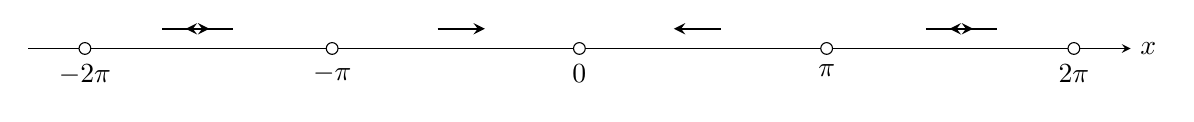
\begin{tikzpicture}[>=stealth, scale=1.0]
  \draw[->] (-7,0) -- (7,0) node[right] {$x$};
  \foreach \x/\lab/\type in {-6.28/$-2\pi$/s, -3.14/$-\pi$/u, 0/$0$/s, 3.14/$\pi$/u, 6.28/$2\pi$/s}{
    \ifx\types\node[circle,fill,inner sep=1.5pt,label=below:{\lab}] at (\x,0) {};
    \else\node[circle,draw,fill=white,inner sep=1.5pt,label=below:{\lab}] at (\x,0) {};\fi
  }
  % Flow arrows: between stable and unstable, flow toward stable
  \foreach \xs in {-5, -1.5, 4.7}{ \draw[->,thick] (\xs-0.3,0.25) -- (\xs+0.3,0.25); }
  \foreach \xs in {-4.7, 1.5, 5}{ \draw[<-,thick] (\xs-0.3,0.25) -- (\xs+0.3,0.25); }
\end{tikzpicture}
\end{center}
Filled circles: stable; open circles: unstable. Flow points toward each $2k\pi$.

\subsection*{(b) $0<r<2$: bifurcations and counting}

Fixed points satisfy $\sin x = rx$. Geometrically: intersections of $y=\sin x$ with the line $y=rx$.

\textbf{Tangent bifurcations.} At each saddle-node, $rx = \sin x$ and $r = \cos x$ tangentially. Eliminate:
\[ \cos x_n\cdot x_n = \sin x_n \;\Rightarrow\; \tan x_n = x_n. \]
Solutions occur near $x_n \approx (n+\tfrac{1}{2})\pi$ for $n=1,2,\dots$ (positive side; symmetric on negative side). Bifurcation values:
\[ r_n = \cos x_n. \]
For small $r$, the tangent bifurcations occur at large $x_n$ where $\tan x \approx x$ gives $x_n \approx (n+\tfrac{1}{2})\pi - 1/[(n+\tfrac{1}{2})\pi]$. Thus
\[ r_n = \cos x_n \approx (-1)^n\sin\!\left(\frac{1}{(n+\tfrac{1}{2})\pi}\right) \approx \frac{(-1)^n}{(n+\tfrac{1}{2})\pi}. \]
Take absolute values for $r>0$:
\[ \boxed{\;r_n \approx \frac{1}{(n+\tfrac{1}{2})\pi},\quad n=1,2,\dots.\;} \]

\textbf{Counting fixed points.} For $0<r\ll 1$, the line $y=rx$ intersects $\sin x$ near each maximum/minimum of $\sin x$ on $|x|\lesssim 1/r$. Number of crossings:
\[ N(r) \sim \frac{2/r}{\pi} = \frac{2}{\pi r}. \]
\[ \boxed{\;N(r) \approx 2/(\pi r) \text{ for } 0<r\ll 1.\;} \]
At $r=1$: line tangent to $\sin x$ at origin from above; the line touches $\sin x$ only at $x=0$ (one fixed point). For $r>1$ the line is steeper than $\sin x$ near $0$, only one fixed point ($x=0$, unstable since $f'(0)=r-1>0$). At each $r=r_n$ a saddle-node pair annihilates as $r$ increases, until at $r=1$ all extra pairs are gone. For $r=2$: still one fixed point ($x=0$, unstable).

Stability: at $x=0$, $f'(0) = r - 1$. So $x=0$ is stable for $r<1$, unstable for $r>1$. (At $r=1$ a transcritical-like change with the neighbouring pair occurs.) Pairs born in saddle-nodes alternate stable/unstable.

\subsection*{(c) Imaginary-axis dynamics}

Substitute $x\mapsto iy$ ($y\in\mathbb R$):
\[ i\dot y = r(iy) - \sin(iy) = iry - i\sinh y. \]
Divide by $i$:
\[ \dot y = ry - \sinh y. \]
Fixed points: $\sinh y = ry$.

For $r\le 1$: $\sinh y > ry$ for $y>0$ (since $\sinh y \ge y \ge ry$ with equality only at $y=0$), only $y=0$ is a fixed point. Stability: $f'(0) = r - \cosh 0 = r - 1$. Stable for $r<1$, unstable for $r>1$.

For $r>1$: $\sinh y$ grows faster than $ry$ at large $|y|$, but at origin $\sinh y \approx y < ry$, so two new symmetric fixed points $\pm y_*(r)$ appear (pitchfork at $r=1$).

\textbf{Bifurcation diagram} (supercritical pitchfork at $r=1$):

\begin{center}
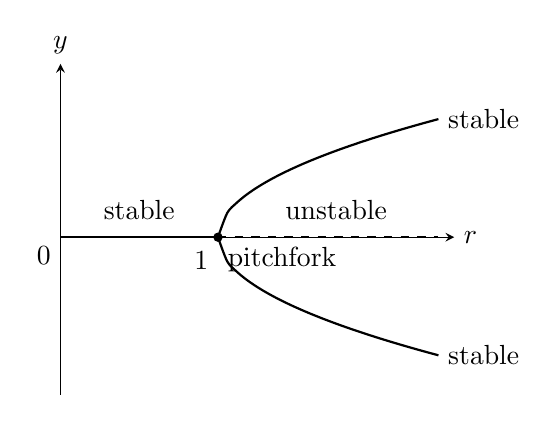
\begin{tikzpicture}[>=stealth, scale=1.0]
  \draw[->] (0,0) -- (5,0) node[right] {$r$};
  \draw[->] (0,-2) -- (0,2.2) node[above] {$y$};
  \node[below left] at (0,0) {$0$};
  \draw[dashed] (2,-0.05) -- (2,0.05) node[below=10pt,left] {$1$};
  % Stable y=0 for r<1: solid line
  \draw[thick] (0,0) -- (2,0);
  % Unstable y=0 for r>1: dashed
  \draw[thick, dashed] (2,0) -- (4.8,0);
  % Two stable branches y_*(r) for r>1
  \draw[thick, domain=2:4.8, smooth, variable=\r] plot ({\r}, { 1.5*sqrt((\r-2)/2.8) });
  \draw[thick, domain=2:4.8, smooth, variable=\r] plot ({\r}, {-1.5*sqrt((\r-2)/2.8) });
  \node[right] at (4.8, 1.5) {stable};
  \node[right] at (4.8,-1.5) {stable};
  \node[above] at (1, 0.1) {stable};
  \node[above] at (3.5, 0.1) {unstable};
  \node[circle,fill,inner sep=1.2pt] at (2,0) {};
  \node[below right] at (2,0) {pitchfork};
\end{tikzpicture}
\end{center}

\subsection*{(d) Phase portrait of the 2D system}

\textbf{Problem.} $\dot x = y^3 - y$, $\dot y = x - y^2$.

\textbf{Fixed points.} Set $\dot x=\dot y=0$:
\[ y(y^2-1) = 0,\qquad x = y^2. \]
First gives $y \in \{0,\pm 1\}$.
\[ y=0:\ x=0. \]
\[ y=\pm 1:\ x=1. \]
Three fixed points: $P_0=(0,0)$, $P_+=(1,1)$, $P_-=(1,-1)$.

\textbf{Jacobian.}
\[ \mathsf J = \begin{pmatrix} 0 & 3y^2-1 \\ 1 & -2y \end{pmatrix}. \]

At $P_0=(0,0)$:
\[ \mathsf J_0 = \begin{pmatrix} 0 & -1 \\ 1 & 0 \end{pmatrix}. \]
Trace $\tau=0$, det $\Delta = 1$. Eigenvalues $\pm i$: \emph{centre} (linear). Nonlinear: try Hamiltonian / first integral. Note $\dot x/\dot y = (y^3-y)/(x-y^2)$:
\[ (x-y^2)\,\de x = (y^3-y)\,\de y. \]
This is exact: $\de(\tfrac{x^2}{2} - x y^2) = ?$ Test $\partial_y(x-y^2) = -2y$, $\partial_x(-(y^3-y)) = 0$, not exact directly. Instead seek $H$ with $\dot x = -\partial H/\partial y$, $\dot y = \partial H/\partial x$. Need $-\partial_y H = y^3-y$ and $\partial_x H = x-y^2$:
\[ H = \tfrac{x^2}{2} - x y^2 + \tfrac{y^4}{4} \cdot c?\]
Check $\partial_x H = x - y^2$ \checkmark. $\partial_y H = -2xy + g'(y)$; require $-(-2xy+g'(y)) = y^3 - y$:
\[ 2xy - g'(y) = y^3 - y. \]
But this depends on $x$, so the system is \emph{not} Hamiltonian. The centre of the linearisation is therefore \emph{not} guaranteed.

Compute divergence:
\[ \nabla\cdot\vb f = \partial_x(y^3-y) + \partial_y(x-y^2) = -2y. \]
Non-zero, so phase area is not conserved; near $P_0$ at $y=0$ divergence vanishes to leading order. Linear analysis gives a centre; nonlinear terms decide. We treat $P_0$ as a (nonlinear) centre/focus; the phase portrait shows closed-curve-like trajectories near origin (sketched as a centre below).

At $P_\pm = (1,\pm 1)$:
\[ \mathsf J_\pm = \begin{pmatrix} 0 & 2 \\ 1 & \mp 2 \end{pmatrix}. \]

$P_+$ ($y=1$):
\[ \tau = -2,\quad \Delta = 0\cdot(-2) - 2\cdot 1 = -2. \]
$\Delta<0$: \emph{saddle}. Eigenvalues from $\lambda^2+2\lambda - 2=0$:
\[ \lambda = -1 \pm \sqrt{3}. \]
Eigenvectors: for $\lambda_+ = -1+\sqrt 3$, $(\mathsf J_+ - \lambda_+ I)\vb v=0$:
\[ -\lambda_+ v_1 + 2 v_2 = 0 \;\Rightarrow\; \vb v_+ \propto (2,\lambda_+) = (2,\sqrt 3-1). \]
For $\lambda_- = -1-\sqrt 3$: $\vb v_- \propto (2,-\sqrt 3-1)$.

$P_-$ ($y=-1$):
\[ \tau = +2,\quad \Delta = 0\cdot(2) - 2\cdot 1 = -2. \]
$\Delta<0$: \emph{saddle}. Eigenvalues from $\lambda^2-2\lambda-2=0$:
\[ \lambda = 1 \pm \sqrt 3. \]

\textbf{Nullclines.}
\[ \dot x = 0:\quad y=0,\ y=\pm 1\ \text{(horizontal lines)}. \]
\[ \dot y = 0:\quad x = y^2\ \text{(parabola opening right)}. \]
Saddles sit on parabola at $y=\pm 1$; centre at origin.

\textbf{Phase portrait.}

\begin{center}
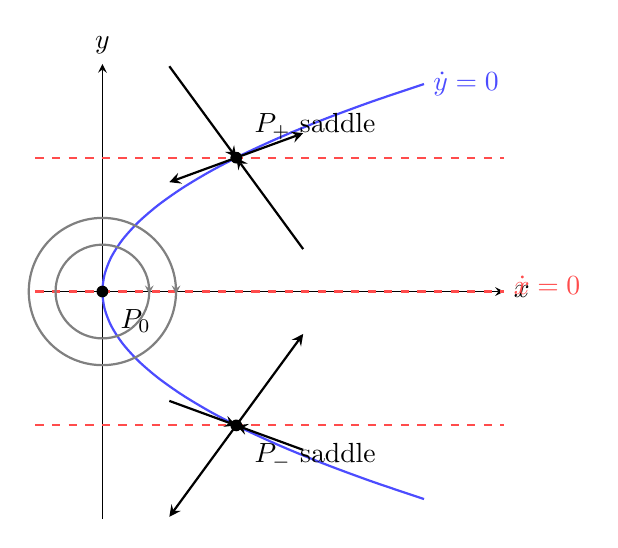
\begin{tikzpicture}[>=stealth, scale=1.7]
  % axes
  \draw[->] (-0.5,0) -- (3.0,0) node[right] {$x$};
  \draw[->] (0,-1.7) -- (0,1.7) node[above] {$y$};
  % parabola x=y^2
  \draw[thick, domain=-1.55:1.55, smooth, variable=\t, blue!70] plot ({\t*\t}, {\t});
  \node[blue!70, right] at (2.4,1.55) {$\dot y=0$};
  % horizontal lines y=0,\pm1
  \draw[thick, red!70, dashed] (-0.5,1) -- (3,1);
  \draw[thick, red!70, dashed] (-0.5,-1) -- (3,-1);
  \draw[thick, red!70, dashed] (-0.5,0) -- (3,0);
  \node[red!70, right] at (3,0.05) {$\dot x=0$};
  % fixed points
  \node[circle,fill,inner sep=1.5pt,label={[label distance=2pt]below right:{$P_0$}}] at (0,0) {};
  \node[circle,fill,inner sep=1.5pt,label={[label distance=2pt]above right:{$P_+$ saddle}}] at (1,1) {};
  \node[circle,fill,inner sep=1.5pt,label={[label distance=2pt]below right:{$P_-$ saddle}}] at (1,-1) {};
  % saddle separatrices at P_+
  \draw[->,thick] (1,1) -- ++(0.5,{0.5*(sqrt(3)-1)/2});
  \draw[->,thick] (1,1) -- ++(-0.5,{-0.5*(sqrt(3)-1)/2});
  \draw[<-,thick] (1,1) -- ++(0.5,{0.5*(-sqrt(3)-1)/2});
  \draw[<-,thick] (1,1) -- ++(-0.5,{-0.5*(-sqrt(3)-1)/2});
  % saddle separatrices at P_-
  \draw[->,thick] (1,-1) -- ++(0.5,{0.5*(1+sqrt(3))/2});
  \draw[->,thick] (1,-1) -- ++(-0.5,{-0.5*(1+sqrt(3))/2});
  \draw[<-,thick] (1,-1) -- ++(0.5,{0.5*(1-sqrt(3))/2});
  \draw[<-,thick] (1,-1) -- ++(-0.5,{-0.5*(1-sqrt(3))/2});
  % closed orbits around origin (centre-like)
  \draw[thick, gray] (0,0) ellipse (0.35 and 0.35);
  \draw[thick, gray] (0,0) ellipse (0.55 and 0.55);
  % flow arrows on the orbits
  \draw[->,gray] (0.35,0.02) -- (0.35,-0.02);
  \draw[->,gray] (0.55,0.02) -- (0.55,-0.02);
\end{tikzpicture}
\end{center}

Summary:
\[ \boxed{\;P_0=(0,0)\text{ centre (linear)},\quad P_\pm=(1,\pm 1)\text{ saddles}.\;} \]

%=====================================================================
\section*{Question 4 --- Stochastic gene expression}
%=====================================================================

\subsection*{(a) Deterministic solutions and steady states}

\textbf{Problem.} Solve $\dot R = k_R - \gamma_R R$, $\dot P = k_P R - \gamma_P P$ for $R(t)$ and steady states.

Linear ODE for $R$:
\[ \dot R + \gamma_R R = k_R. \]
General solution:
\[ R(t) = \frac{k_R}{\gamma_R} + \!\left(R_0 - \frac{k_R}{\gamma_R}\right)\!e^{-\gamma_R t}. \]
\[ \boxed{\;R(t) = \frac{k_R}{\gamma_R}\!\left(1-e^{-\gamma_R t}\right) + R_0 e^{-\gamma_R t}.\;} \]

Steady state: $\dot R = 0$:
\[ \langle R\rangle_{ss} = \frac{k_R}{\gamma_R}. \]
Then $\dot P = 0$:
\[ \langle P\rangle_{ss} = \frac{k_P}{\gamma_P}\langle R\rangle_{ss} = \frac{k_P k_R}{\gamma_P\gamma_R}. \]
\[ \boxed{\;\langle R\rangle_{ss} = k_R/\gamma_R,\qquad \langle P\rangle_{ss} = k_P k_R/(\gamma_P\gamma_R).\;} \]

\textbf{Numerical estimate.} Transcribed in $1$~min: $k_R = 1$ molecule/min. RNA lifetime $1/\gamma_R = 10$~min, so $\gamma_R = 0.1$~min$^{-1}$:
\[ \langle R\rangle_{ss} = 1/0.1 = 10. \]
\[ \boxed{\;\langle R\rangle_{ss} \approx 10\text{ RNA molecules per cell.}\;} \]

\subsection*{(b) Mean-square fluctuations in $R$}

Linearise about the steady state: $R = \langle R\rangle + \delta R$, drive by noise $\eta_R(t)$:
\[ \delta\dot R = -\gamma_R\,\delta R + \eta_R(t). \]
Fourier transform $\delta R(t) = \int\!\frac{\de\omega}{2\pi}\,\delta\tilde R(\omega) e^{-i\omega t}$:
\[ -i\omega\,\delta\tilde R = -\gamma_R\,\delta\tilde R + \tilde\eta_R. \]
Solve:
\[ \delta\tilde R(\omega) = \frac{\tilde\eta_R(\omega)}{\gamma_R - i\omega}. \]
Power spectrum from $\langle\eta_R(t)\eta_R(t-t')\rangle = q_R\delta(t')$:
\[ \langle\tilde\eta_R(\omega)\tilde\eta_R^*(\omega')\rangle = 2\pi q_R\,\delta(\omega-\omega'). \]
Hence
\[ \langle|\delta\tilde R(\omega)|^2\rangle = \frac{q_R}{\gamma_R^2 + \omega^2}\cdot 2\pi\delta(0)_{\omega=\omega'}. \]
By Wiener--Khinchin:
\[ \langle\delta R^2\rangle = \int_{-\infty}^{\infty}\!\frac{\de\omega}{2\pi}\,\frac{q_R}{\gamma_R^2+\omega^2}. \]
Apply standard integral with $a=\gamma_R$:
\[ \int_{-\infty}^{\infty}\!\frac{\de\omega}{2\pi(\omega^2+\gamma_R^2)} = \frac{1}{2\gamma_R}. \]
Therefore
\[ \boxed{\;\langle\delta R^2\rangle = \frac{q_R}{2\gamma_R}.\;} \]

\subsection*{(c) Fano factor for $P$}

Given
\[ \langle\delta P^2\rangle = \langle P\rangle\!\left(1 + \frac{k_P}{\gamma_R+\gamma_P}\right). \]
Fano factor:
\[ F = \frac{\langle\delta P^2\rangle}{\langle P\rangle} = 1 + \frac{k_P}{\gamma_R+\gamma_P}. \]
Manipulate: factor $\gamma_R$ from denominator:
\[ F = 1 + \frac{k_P/\gamma_R}{1 + \gamma_P/\gamma_R}. \]
Identify
\[ b = \frac{k_P}{\gamma_R},\qquad \phi = \frac{\gamma_P}{\gamma_R}. \]
\[ \boxed{\;F = 1 + \frac{b}{1+\phi}.\;} \]

\textit{Interpretation.}
\begin{itemize}
\item $b = k_P/\gamma_R$: \emph{burst size} --- average number of protein molecules produced from a single mRNA before it is degraded (translation rate $\times$ mRNA lifetime).
\item $\phi = \gamma_P/\gamma_R$: ratio of protein-to-mRNA degradation rates. Since mRNA is much less stable than protein, $\gamma_R \gg \gamma_P$, so $\phi\ll 1$.
\end{itemize}
\textit{Poissonian limit.} Pure Poisson ($b=0$, no bursting): $F=1$.

\textit{Dependence on $k_P$.} With $\phi\ll 1$ ($1+\phi\approx 1$),
\[ F \approx 1 + b = 1 + k_P/\gamma_R. \]
$F$ grows linearly in the translation rate $k_P$.

\begin{center}
\begin{tikzpicture}[>=stealth, scale=1.0]
  \draw[->] (0,0) -- (5,0) node[right] {$k_P$};
  \draw[->] (0,0) -- (0,3.5) node[above] {$F$};
  \draw[dashed] (0,1) -- (5,1);
  \node[left] at (0,1) {$1$};
  \draw[thick, domain=0:4.7, smooth, variable=\k] plot (\k, {1 + 0.5*\k});
  \node[right] at (4.7, 3.4) {$F = 1 + k_P/\gamma_R$};
  \node[circle,fill,inner sep=1.2pt,label=below left:{$F=1$}] at (0,1) {};
\end{tikzpicture}
\end{center}

Larger $k_P$ produces more proteins per mRNA burst, so the variance grows super-Poissonian; bursting is the source of the excess noise.

\subsection*{(d) Intrinsic vs.\ extrinsic noise}

\textit{Intrinsic noise.} Stochastic fluctuations originating from the inherent randomness of biochemical reactions (transcription, translation, degradation) within a single cell, given fixed cellular conditions. It is independent across two identical reporter genes in the same cell.

\textit{Extrinsic noise.} Fluctuations arising from cell-to-cell differences in shared cellular factors (RNA polymerase, ribosome counts, cell volume, metabolic state). It correlates the expression of two reporter genes in the same cell.

\textit{Beneficial roles of intrinsic noise.}
\begin{itemize}
\item \emph{Phenotypic diversity / bet-hedging}: a clonal population samples multiple expression states, raising the chance that some cells survive sudden environmental change (e.g.\ bacterial persistence).
\item \emph{Stochastic differentiation}: in development or competence switching (e.g.\ \emph{B.\ subtilis} competence), noise breaks symmetry between cells and triggers cell-fate decisions.
\end{itemize}

\textit{Detrimental roles.}
\begin{itemize}
\item \emph{Loss of fidelity}: noisy expression of essential housekeeping proteins compromises homeostasis.
\item \emph{Disease}: stochastic mis-regulation contributes to oncogenic states and developmental defects.
\item \emph{Reduced precision}: noise limits the accuracy of signalling, sensing, and gene-regulatory circuit responses.
\end{itemize}

\end{document}
